Building upon the physics-informed and hybrid paradigms discussed in Section~\ref{sec:drl_design_trends}, 
the control stage translates these algorithmic insights into real-time decision-making and adaptive regulation for PECs. 
While the design phase establishes structural and parametric foundations, 
the control phase governs dynamic behavior, resilience, and online optimization. 
In this context, DRL has emerged as a powerful paradigm for intelligent control, 
offering model-free, adaptive policy learning under nonlinear and time-varying conditions. 
Unlike conventional schemes relying on fixed models or rule-based tuning, DRL controllers continuously interact with the environment to optimize long-term performance under uncertainty. 
This section reviews recent progress in DRL-enabled converter control, 
focusing on two major methodologies: \textit{independent DRL control}, where DRL directly governs converter dynamics, 
and \textit{hybrid DRL control}, where DRL interacts with conventional control frameworks through parameter tuning, nonlinear compensation, or time-segmented coordination to enhance adaptability and robustness.



\subsection{Independent Control of PECs}
\label{sec:ctrl_direct}

\begin{figure}[!t]
    \centering
    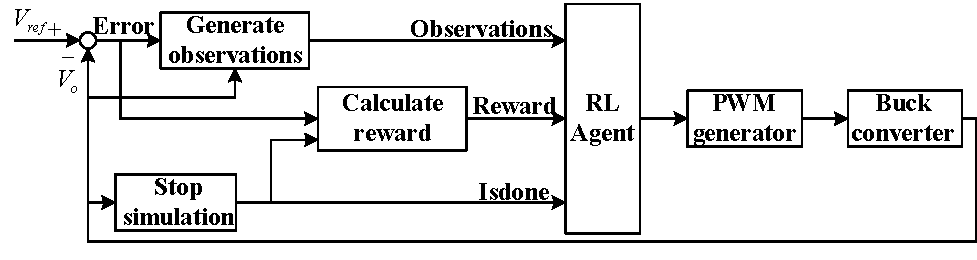
\includegraphics[width=0.95\linewidth]{fig/control1111.pdf} 
    \caption{Control strategy for the Buck converter with independent DRL control \cite{9752938}.}
    \label{fig:control9}
\end{figure}

In the control domain of PECs, the direct deployment of DRL has demonstrated strong potential in addressing nonlinear dynamics, parameter uncertainties, and time-varying operating conditions. Unlike conventional controllers based on explicit models or predefined rules, DRL agents autonomously learn optimal policies through interaction with the system environment, achieving adaptive and model-free control across diverse converter topologies.

For \textbf{non-isolated DC-DC converters} such as Buck and Boost converters, DRL methods primarily focus on generating duty cycles or their increments directly from observed system states. Studies \cite{9660319, 9752938, 10030117,9521987, zandi2023voltage, 10245391, 10264605, 10246775,chen2024asynchronous,li2023large} have systematically explored DRL-based independent control strategies for Buck converters, using algorithms such as DQN, DDQN, DDPG, and NAF. A typical control block diagram is presented in Fig.~\ref{fig:control9}, which shows an independent RL control strategy that controls the output voltage of a buck converter. For instance, \cite{9660319} proposes a curriculum learning approach by integrating a goal proposal module with DDQN to improve convergence speed. The sensitivity of hyperparameters and reward function designs is analyzed in \cite{9521987}, revealing that minor variations have limited impact on control performance. In \cite{10264605}, a trade-off between state space completeness and convergence speed is discussed, and reward shaping techniques are shown to influence overshoot and steady-state error. The NAF-based control in \cite{10246775} further demonstrates that a linear reward function achieves superior convergence, while state space augmentation with filtered current derivatives improves training effectiveness.

Bidirectional Buck/Boost converters have also been studied using TD3-based DRL strategies \cite{10141314}, where the agent directly determines switching actions to regulate power bidirectionally. For SIMO topologies, \cite{ye2024deep} introduces a DDPG-based control framework that efficiently decouples multi-port outputs using a single inductor. This method outperforms adaptive and deadbeat controllers in dynamic response and sensor reduction.

In the context of cascaded systems, \cite{anugula2021deep} adopts DDPG for speed control of a Buck-fed DC motor, generating duty ratios in real-time. A quasi-Z-source converter is addressed in \cite{zandi2023voltage} using a discrete-action RL agent, simplifying network design and accelerating convergence while reducing memory usage.

For \textbf{isolated DC-DC converters} such as DAB and CLLLC resonant topologies, DRL agents shift from duty cycle control to regulating phase shift angles. In \cite{wu2021innovative}, DDPG is applied to generate phase modulation strategies in DAB converters, achieving enhanced soft-switching performance and reduced circulating current, which are critical for high-efficiency operation.

In DC-AC applications, such as inverters and electric drives, DRL strategies enable end-to-end control of voltage and current outputs without requiring explicit model identification 


\begin{table*}[t]
\centering
\caption{Summary of Selected Independent DRL Control Strategies for PECs}
\label{tab:independent_control_summary}
\renewcommand{\arraystretch}{1.25}
\resizebox{\textwidth}{!}{
\begin{tabular}{@{}p{3.3cm} p{4.3cm} p{1.8cm} l p{5.8cm}@{}}
\toprule
\textbf{Converter Type} & \textbf{Control Target} & \textbf{Algorithm} & \textbf{Reference} & \textbf{Advantage (+) and Disadvantage (-)} \\ 
\midrule

Buck / Boost / Buck-Boost &
Voltage regulation via duty ratio &
DQN, DDQN, \newline
DDPG, A3C, \newline
MADDPG &
\cite{9660319,9752938,10030117,9521987,zandi2023voltage,10245391,10264605,10246775,chen2024asynchronous,li2023large} &
+ Adaptive to disturbances \newline
+ No model required \newline
- Reward-sensitive convergence \newline
- High training cost \\ 
\midrule

Bidirectional Buck/Boost &
Bidirectional power flow control &
TD3 &
\cite{10141314} &
+ Suitable for nonlinear bidirectional power paths \newline
- Sensitive to policy tuning \newline
- High parameter sensitivity \\ 
\midrule

SIMO DC-DC &
Multi-output decoupling control &
DDPG &
\cite{ye2024deep} &
+ Handles multi-input-multi-output systems \newline
+ Requires fewer sensors \newline
- Scalability challenges \newline
- Training time increases with outputs \\ 
\midrule

DC Motor (Buck / Quasi-Z) &
Speed control under nonlinear dynamics &
DDPG &
\cite{anugula2021deep} &
+ Learns nonlinear motor dynamics \newline
+ Eliminates model dependency \newline
- Convergence depends on abstraction accuracy \newline
- High tuning effort \\ 
\midrule

Isolated DC-DC (DAB / CLLLC) &
Phase-shift and ZVS control &
DDPG &
\cite{wu2021innovative} &
+ Guarantees ZVS operation \newline
+ Provides flexible regulation capability \newline
- Coupled control adds design complexity \newline
- Computationally demanding \\ 
\midrule

DC-AC (NPC / PMSM) &
Current or voltage tracking &
DDPG, DQN, PPO, \newline
MADDPG &
\cite{book2021transferring,schenke2021deep,traue2020toward,qashqai2023model,weber2023steady,yan2022multiagent,pinthurat2023simultaneous} &
+ Learns control law without PLL dependency \newline
+ Handles nonlinear current and voltage profiles \newline
- Sensitive to sensor noise \newline
- Reward design requires fine-tuning \\ 
\midrule

Renewable Energy Systems (PV / Wind / WEC) &
MPPT and stability enhancement &
QL, DQN, \newline
TD3, \newline
Quantum DRL &
\cite{wei2015reinforcement,arianborna2023mppt,kosuru2022deep,yin2021quantum,zou2022optimization,chen2024control} &
+ Outperforms classical P\&O in MPPT tasks \newline
+ Adapts to stochastic wind or sea-state variations \newline
+ Suppresses low-frequency oscillations \newline
- Algorithmic complexity \newline
- Limited hardware validation \\ 
\midrule

MMC / ISOP-DAB &
Module coordination and voltage balancing &
PG, MASAC, \newline
MATD3, DQN &
\cite{jiang2021application,jung2022reinforcement,zeng2021deep,zeng2022multiagent,zeng2022autonomous,zeng2023deep} &
+ Enables scalable modular control \newline
+ Supports distributed and autonomous operation \newline
- Distributed training still under development \newline
- Communication delay impacts stability \\ 
\bottomrule
\end{tabular}}
\end{table*}




\noindent
or reference tracking. Studies \cite{book2021transferring, schenke2021deep, traue2020toward, qashqai2023model, weber2023steady, yan2022multiagent,pinthurat2023simultaneous} apply DDPG, DQN, and PPO to motor drives and multilevel inverters. For example, \cite{schenke2021deep} proposes a DQN-based torque control strategy that segments the operating space of PMSMs and designs region-specific reward functions, leading to robust performance without the need for motor parameters. \cite{qashqai2023model} presents a DQN-based control method for NPC inverters, showing improved resilience to parameter variations and sensor noise. To enhance steady-state performance, \cite{weber2023steady} introduces a reward compensation scheme using integral action augmentation, which can be applied across actor-critic-based RL controllers.

Beyond conventional DC-DC and DC-AC applications, DRL has been increasingly adopted in renewable energy systems for maximum power point tracking (MPPT) and stability enhancement. For instance, Q-learning and its deep variants have been applied to PV systems to design adaptive MPPT controllers that outperform classical perturb-and-observe schemes by achieving faster convergence and reduced oscillations around the maximum power point~\cite{wei2015reinforcement}. Similarly, a DQN-based MPPT strategy for permanent-magnet synchronous generator (PMSG) wind turbines demonstrates improved dynamic tracking under stochastic wind speed variations~\cite{arianborna2023mppt}. More advanced works further integrate DRL with stability-oriented objectives: Q-learning and TD3 controllers have been developed to suppress low-frequency oscillations in doubly-fed induction generator (DFIG)-based systems, while quantum deep reinforcement learning has been proposed to enhance the rotor-side converter performance under severe disturbances~\cite{kosuru2022deep,yin2021quantum}. Collectively, these studies highlight the capacity of DRL to extend independent control paradigms toward renewable-driven systems, where adaptivity and robustness against environmental variability are critical. Beyond PV and wind energy systems, DRL has also been explored in ocean wave energy converters (WECs)~\cite{yang2020deep,chen2024control}, where model-free DRL controllers outperform linear reactive controllers under irregular sea states, achieving up to 152\% improvement in energy capture. These works collectively demonstrate that independent DRL control extends seamlessly from classical DC-DC converters to complex renewable-driven infrastructures, highlighting its adaptability in highly uncertain environments.


For complex modular topologies like MMCs and ISOP-DAB converters, DRL offers scalable solutions to high-dimensional control problems. In \cite{jiang2021application}, a PG-based framework is proposed for MMCs, optimizing current control and capacitor balancing through multi-objective reward design. \cite{jung2022reinforcement} applies DQN to develop near-level modulation (NLM), mitigating thermal imbalances across modules. Multi-agent approaches are introduced in \cite{zeng2021deep, zeng2022multiagent, zeng2022autonomous,zeng2023deep}, where each submodule in ISOP-DAB is treated as an autonomous agent coordinated by algorithms such as MADDPG, MASAC, and MATD3. These architectures support distributed voltage balancing, current sharing, and redundancy, and are experimentally validated using microcontroller-based implementations.

Overall, DRL-based independent control provides a flexible and unified control paradigm capable of adapting to a wide variety of converter structures. As summarized in Table~\ref{tab:independent_control_summary}, these methods demonstrate strong generalization across voltage regulation, current tracking, and power balancing tasks. Despite promising results, real-time applicability, training stability, and reward design remain critical challenges, encouraging continued exploration into hybrid and safety-constrained DRL frameworks.

\subsection{Hybrid Control of PECs}
\label{sec:ctrl_hybrid}
In addition to the independent control methods, DRL can also be incorporated as an enhancement to traditional control strategies, forming hybrid control architectures. Hybrid control leverages the strengths of both conventional controllers and DRL to improve the overall performance of PECs in real-world applications. This approach is particularly beneficial for PECs with complex dynamics, where traditional methods may be limited in adaptability or computational efficiency. The hybrid control method typically involves three primary strategies: tuning the control parameters of traditional strategies, compensating traditional control strategies, and combining DRL algorithms with traditional strategies in a time-segmented manner. 

%%%%%%%%%%%%%%%%%%%%%%%%%%%%%%%%%%%%%%%%%%%%%%%%%%%
\subsubsection{Parameter Tuning of Conventional Controllers}
%%%%%%%%%%%%%%%%%%%%%%%%%%%%%%%%%%%%%%%%%%%%%%%%%%%
When integrated into conventional control loops, DRL enables dynamic tuning of parameters such as feedback gains, prediction horizons, and modulation indices, thus enhancing the adaptability, stability, and control performance of PECs without explicit modeling. This approach is especially beneficial in scenarios where traditional controllers suffer from limited adaptability under time-varying disturbances or parameter uncertainties.

In \textbf{non-isolated DC-DC converters}, such as Buck, Boost, and Buck-Boost topologies, DRL has been extensively used to tune classical control strategies like PI, ADRC, LQR, GPC, and MPC. For Buck converters, studies~\cite{gheisarnejad2020iot,teng2020reinforcement,alfred2021model,dong2022generalized} demonstrate the use of DDPG, ADP, and TD3 to adaptively tune parameters of nonlinear feedback controllers, LQR, and GPC schemes. These methods improve dynamic performance by adjusting control gains in real time based on environmental feedback. In Boost converters, PPO, DDQN, and DDPG algorithms have been applied to tune model-free sliding mode controllers~\cite{gheisarnejad2022reducing}, PI coefficients~\cite{mao2022research}, and predictive horizons~\cite{khooban2022smartenance,cui2023adaptive}, respectively. Notably,~\cite{huangfu2022learning} employs a high-order sliding mode observer (SMO) for uncertainty estimation, with DDPG adjusting the gains accordingly to accelerate the response.


\begin{figure}[!t]
    \centering
    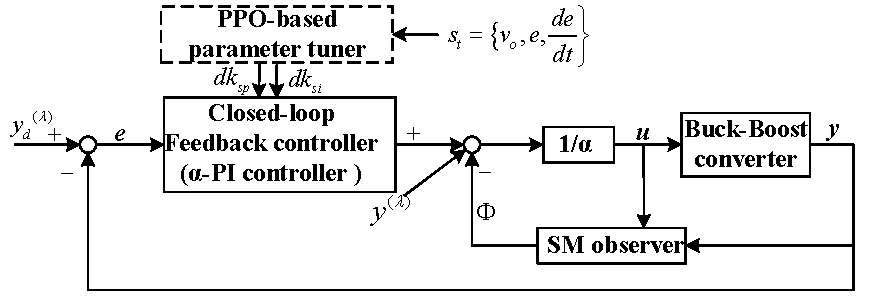
\includegraphics[width=0.95\linewidth]{fig/control1112.pdf} 
    \caption{Control strategy for Buck-Boost converter with PPO tuning ULM controller \cite{hajihosseini2020dc}.}
    \label{fig:control5}
\end{figure}



\begin{table*}[t]
\centering
\caption{Summary of DRL-Tuned Traditional Control Strategies for PECs}
\label{tab:drl_tuning_summary}
\renewcommand{\arraystretch}{1.25}
\resizebox{\textwidth}{!}{
\begin{tabular}{@{}p{2.3cm} p{3.3cm} p{3.3cm} l p{6.8cm}@{}}
\toprule
\textbf{Converter Type} & \textbf{Control Target} & \textbf{Algorithm} & \textbf{Reference} & \textbf{Advantage (+) and Disadvantage (-)} \\ 
\midrule

Buck / Boost \newline / Buck-Boost &
Adaptive tuning of PID, ADRC, or MPC controllers &
DDPG, TD3, PPO, QL, DDQN &
\cite{gheisarnejad2020iot,teng2020reinforcement,alfred2021model,dong2022generalized,gheisarnejad2022reducing,mao2022research,khooban2022smartenance,cui2023adaptive,huangfu2022learning} &
+ Strong adaptability to operating conditions \newline
+ Enhanced dynamic performance without manual tuning \newline
- Complex reward and state-space design \newline
- High training cost and data requirements \\ 
\midrule

Isolated DC-DC \newline (e.g., DAB) &
Modulation and frequency tuning for efficiency improvement &
QL, DDPG, TD3 &
\cite{mahazabeen2022performance,tang2020reinforcement,tang2021deep,tang2022deep} &
+ Achieves full-range efficiency enhancement \newline
+ Maintains robustness under fault conditions \newline
- Requires extensive offline training \newline
- Limited performance with discrete Q-learning \\ 
\midrule

DC-AC Inverter &
Adaptive feedback and MPC gain tuning &
TD3, SAC, DDPG, IRL, MAPPO &
\cite{dragoun2019adaptive,he2021weighting,wan2021reinforcement,jiang2023stability,liang2022multiagent,fathollahi2023robust,qie2023new,bo2022controller} &
+ Improves system stability and disturbance rejection \newline
+ Adapts effectively to parameter uncertainties \newline
- Reward shaping is challenging \newline
- Real-time deployment remains computationally intensive \\ 
\midrule

MMC / Interleaved Boost &
Optimal gain tuning for PI control &
IRL + PI &
\cite{qie2022new} &
+ Low computational burden suitable for modular systems \newline
+ Compatible with hierarchical control frameworks \newline
- Limited generalization across converter types \newline
- Requires predefined system modeling \\ 
\bottomrule
\end{tabular}}
\end{table*}

In \textbf{isolated DC-DC converters}, particularly DAB converters, adaptive tuning of phase shift modulation parameters via DRL is shown to enhance efficiency, soft switching, and dynamic power delivery. DDPG and QL algorithms are employed in~\cite{mahazabeen2022performance, tang2020reinforcement, tang2021deep} to adjust PI gains and optimize TPS modulation schemes. While offline Q-table-based QL suffers from discrete state-action limitations, its performance is enhanced by ANN mapping~\cite{tang2021deep} or replaced with continuous-action algorithms for real-time adaptability. TD3 further extends this approach by co-optimizing switching frequency and modulation indices~\cite{tang2022deep}, reducing converter losses across broad operating conditions.

In \textbf{DC-AC converters}, DRL-assisted parameter tuning addresses challenges related to component aging, uncertain grid conditions, and controller overparameterization. For LCL-filtered inverters, RL is used to adaptively adjust optimal feedback gains, ensuring stability even under actuator saturation and LCL uncertainty~\cite{dragoun2019adaptive}. In three-phase inverters, DDPG tunes the weighting factors in MPC controllers~\cite{he2021weighting,wan2021reinforcement}, while for grid-tied converters, DDPG adjusts PI loop gains with phase margin consideration to improve closed-loop robustness~\cite{jiang2023stability,liang2022multiagent}. Additionally, SAC~\cite{fathollahi2023robust} and IRL~\cite{qie2023new} methods are introduced for tuning control laws in full-bridge converters with CPLs. A comparative evaluation in~\cite{bo2022controller} underscores the tradeoff between fully autonomous and hybrid tuning strategies, indicating that RL-tuned classical control can achieve competitive performance with lower training overhead.

In \textbf{modular topologies}, such as interleaved Boost converters and MMCs, intelligent robust control schemes leverage IRL or DDPG to adapt control gains in real time. For example,~\cite{qie2022new} proposes a hybrid control architecture combining optimal control, PI compensation, and IRL, where the PI loop handles inter-module mismatch and IRL enables online gain adaptation. These designs significantly reduce computational cost while maintaining high dynamic tracking precision, positioning DRL-based tuning as a practical solution for scalable, modular converter control. 

To reduce parameter dependence and improve generalization across varying operating conditions, hybrid frameworks combining SMO, ultra-local modeling (ULM), and DRL are also proposed. An illustrative example of this parameter-tuning paradigm is shown in Fig.~\ref{fig:control5}, where a PPO agent dynamically adjusts the parameters of an ULM controller for a Buck--Boost converter, 
resulting in reduced overshoot and faster convergence compared with conventional tuning. For instance,~\cite{hajihosseini2020dc} integrates PPO with intelligent PI (iPI) control to address instability under CPLs. These approaches exhibit superior convergence and robustness but require careful reward shaping and state space engineering. 

Beyond converter-level parameter adaptation, hybrid DRL strategies have also been extended to system-level control tasks. For example, in microgrid applications, a DRL-assisted reserve control framework for PV systems dynamically determines the reserve ratio and duty cycle, enabling effective frequency regulation under stochastic irradiance and load variations~\cite{zhou2023ai}. In the automotive domain, reinforcement learning-based energy management strategies for hybrid energy storage systems (HESSs) have been proposed to coordinate batteries and supercapacitors, thereby improving energy efficiency and extending battery lifetime in EVs~\cite{ranjbaran2023reinforcement}. These works demonstrate that hybrid DRL control can transcend traditional tuning objectives by embedding system-level reliability and economic considerations, bridging the gap between converter adaptivity and grid-level stability.

The summary of DRL-tuned Traditional Control Strategies for PECs is shown in Table~\ref{tab:drl_tuning_summary}.

%%%%%%%%%%%%%%%%%%%%%%%%%%%%%%%%%%%%%%%%%%%%%%%%%%%
\subsubsection{Parameter Tuning of Conventional Controllers}
%%%%%%%%%%%%%%%%%%%%%%%%%%%%%%%%%%%%%%%%%%%%%%%%%%%

\begin{figure}[!t]
    \centering
    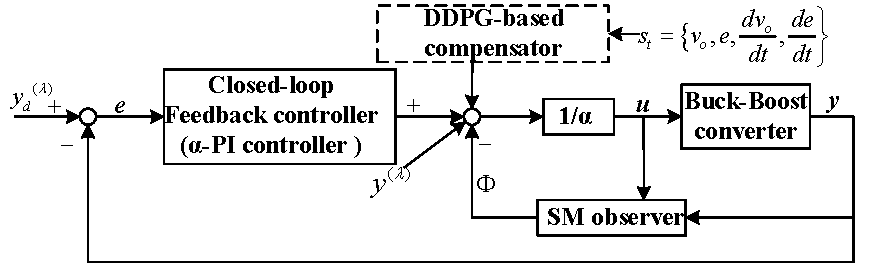
\includegraphics[width=0.95\linewidth]{fig/control1113.pdf} 
    \caption{Control strategy for Buck-Boost converter with DDPG compensating ULM controller \cite{gheisarnejad2020novel}.}
    \label{fig:control4}
\end{figure}


\begin{table*}[t]
\centering
\caption{Summary of DRL-Compensated Hybrid Control Strategies for Power Electronic Converters}
\label{tab:drl_compensation_summary}
\renewcommand{\arraystretch}{1.25}
\resizebox{\textwidth}{!}{
\begin{tabular}{@{}p{2.0cm} p{4.5cm} p{2.0cm} l p{8.0cm}@{}}
\toprule
\textbf{Topology Type} & \textbf{Control Target} & \textbf{Algorithm} & \textbf{Reference} & \textbf{Advantage (+) and Disadvantage (-)} \\ 
\midrule

Buck / Boost \newline  / Buck-Boost &
Nonlinear compensation to PID, SMO-iPI, or MPC controllers for voltage regulation &
DDPG, \newline TD3, PPO &
\cite{hu2021novel,gheisarnejad2020novel,nicola2023improved,lu2021speed} &
+ Adaptive to varying operating conditions \newline
+ Enhances both steady-state and transient performance \newline
- Sensitive to reward and state design \newline
- High computational and training burden \\ 
\midrule

Isolated DC-DC \newline  (e.g., DAB) &
Compensation for modulation indices and soft-switching optimization &
TD3, DDPG &
\cite{lee2023pwm,meng2022novel,chou2019maximum,tang2021rl} &
+ Enables full-range efficiency optimization \newline
+ Maintains resilience under disturbances and faults \newline
- Requires extensive offline training or pretraining \newline
- Discrete Q-learning unsuitable for continuous modulation \\ 
\midrule

DC-AC Inverter &
Compensation to robust control, PI, or MPC schemes for THD and ripple suppression &
TD3, DDPG &
\cite{nicola2022improved,wang2023improved,nicola2022comparative} &
+ Preserves system stability under uncertainties \newline
+ Effective for grid-tied operation with harmonic mitigation \newline
- Real-time reward tuning required for adaptation \newline
- Implementation overhead remains nontrivial \\ 
\bottomrule
\end{tabular}}
\end{table*}


Another common approach in hybrid control is when DRL compensates traditional control strategies. Here, DRL can serve as a nonlinear compensator that enhances the performance of conventional control systems. Acting as an auxiliary layer, DRL dynamically adjusts or corrects the control output based on real-time feedback, particularly under nonlinearities, parameter variations, or disturbances. This scheme retains the interpretability and stability of classical controllers while leveraging the adaptivity of learning-based techniques.

In \textbf{non-isolated DC-DC converters}, DRL-based compensation is extensively applied to Buck, Boost, and Buck-Boost topologies. For Buck converters, DDPG is used to generate nonlinear compensations added to PID or SMO-iPI control outputs~\cite{hu2021novel,gheisarnejad2020novel}. As illustrated in Fig.~\ref{fig:control4}, a DDPG agent operates in parallel with an ULM controller, compensating its output to enhance dynamic voltage regulation under constant-power loads. These frameworks improve adaptability to varying loads and accelerate convergence through reward shaping and stochastic exploration mechanisms. In Boost converters, TD3~\cite{nicola2023improved} enhance traditional PI or MPC schemes by compensating for large-signal disturbances and maintaining DC bus voltage stability. For Buck-Boost converters, Ref.~\cite{gheisarnejad2020novel} replaces PPO-based parameter tuning with DDPG-based output compensation to improve stability under constant power loads. Furthermore, in motor drive applications, Ref.~\cite{lu2021speed} integrates DDPG with PID controllers to improve transient response and steady-state accuracy for Buck-fed DC motors.

In \textbf{isolated DC-DC converters}, particularly dual-active-bridge (DAB) topologies, DRL-based compensation has been extensively explored to enhance modulation performance, soft-switching behavior, and long-term reliability. For instance, TD3 has been employed to generate PWM/PFM control variables alongside traditional phase-shift PI loops~\cite{lee2023pwm}, while also compensating estimation errors in disturbance observers and backstepping controllers~\cite{meng2022novel}, thereby improving voltage tracking and dynamic regulation under wide load variations. Complementary to this, Q-learning-based offline training frameworks have been developed to optimize triple-phase-shift (TPS) modulation across diverse load and voltage ratios, achieving efficiency improvements by discovering non-intuitive operating points~\cite{chou2019maximum}. To further reduce online computational burden, hybrid RL-ANN schemes have been proposed, where ANN inference accelerates RL-trained policy execution to provide real-time optimal phase-shift control, effectively minimizing current stress while preserving soft-switching conditions~\cite{tang2021rl}. Collectively, these compensation strategies demonstrate the versatility of DRL in advancing DAB modulation, offering improved efficiency, robustness, and device longevity beyond the scope of conventional modulation methods.


For \textbf{DC-AC converters}, TD3 compensates robust control strategies by learning from environmental uncertainties~\cite{nicola2022improved,wang2023improved,nicola2022comparative}. These hybrid schemes improve voltage ripple, total harmonic distortion (THD), and transient performance while preserving system robustness. Across topologies, such hybrid DRL-compensated control architectures offer improved tracking precision, noise resilience, and generalization under varying conditions.


The summary of DRL-compensated hybrid control strategies for PECs is shown in Table~\ref{tab:drl_compensation_summary}.


%%%%%%%%%%%%%%%%%%%%%%%%%%%%%%%%%%%%%%%%%%%%%%%%%%%
\subsubsection{Time-Segmented Integration of DRL and Conventional Control}
%%%%%%%%%%%%%%%%%%%%%%%%%%%%%%%%%%%%%%%%%%%%%%%%%%%
\begin{table*}[t]
\centering
\caption{Classification of DRL Control Application Forms in Power Electronic Converters}
\label{tab:rl_control_classification}
\renewcommand{\arraystretch}{1.25}
\resizebox{\textwidth}{!}{
\begin{tabular}{@{}p{3.2cm} p{4.2cm} p{3.8cm} p{2.2cm} p{5.0cm}@{}}
\toprule
\textbf{Application Form} & \textbf{Description} & \textbf{Typical Strategies} & \textbf{Reference} & \textbf{Advantage (+) and Disadvantage (-)} \\ 
\midrule

Independent RL control &
Directly control the converter using sole RL policies without traditional controllers. &
All RL algorithms &
\cite{9660319,9752938,10030117,9521987} &
+ Model-free \newline
+ Generalizable across topologies \newline
+ Eliminates controller modeling \newline
- Requires large training data \newline
- Low interpretability \newline
- Less robust in rare states \\ 
\midrule

\multirow{3}{*}{Hybrid RL control} &
RL tuning: Adjust parameters of traditional controllers using RL. &
ULM + PPO tuning, ADRC + DDPG tuning, GPC + TD3 tuning &
\cite{hajihosseini2020dc,gheisarnejad2020iot,cui2023adaptive} &
+ Enhances adaptivity to disturbances \newline
+ Avoids fixed gain tuning \newline
- Sensitive to reward/state design \newline
- Algorithmic complexity \\ 
\cmidrule(l){2-5}

& RL compensation: Add RL as compensation layer to classical control output. &
PI + DDPG, NDO + TD3, ULM + SMO + DDPG &
\cite{gheisarnejad2020novel,meng2022novel,lu2021speed} &
+ Improves dynamic response \newline
+ Robust against nonlinearities \newline
- Increased system complexity \newline
- Harder to ensure stability \\ 
\cmidrule(l){2-5}

& RL segmented: Use RL and traditional controllers in different time phases. &
PI + PPO / Filter-segmented schemes &
\cite{prag2021data} &
+ Balances RL exploration with traditional control reliability \newline
+ Fast transient response \newline
- Requires clear segmentation logic \newline
- Limited generalization capability \\ 
\bottomrule
\end{tabular}}
\end{table*}


Another promising hybrid control approach combines DRL with traditional control strategies in a time-segmented manner, wherein DRL governs transient or dynamic phases, while conventional controllers ensure steady-state performance. This scheme is particularly suitable for PECs that undergo distinct operating modes, such as rapid load transients or startup phases, which demand adaptive decision-making beyond the scope of fixed-structure controllers.

A typical example is demonstrated in Buck-Boost converters. \cite{prag2021data} proposes a time-segmented hybrid strategy where PPO governs the initial dynamic phase until the system state reaches its target, after which control is handed off to a PI regulator. Compared to pure PI or DRL control, this hybrid strategy reduces overshoot and improves convergence time. Moreover, incorporating a filtering mechanism during the switching phase further improves control smoothness and long-term stability. Despite the added complexity in reward function tuning and controller coordination, time-segmented DRL hybrid control offers improved adaptability, reduced modeling requirements, and effective management of multi-objective performance constraints in nonlinear converter systems.

DRL-based control strategies significantly enhance PEC performance by adapting to dynamic conditions. Independent RL control directly governs converters, while hybrid methods fine-tune or compensate traditional controllers. A time-segmented approach combines both, offering flexibility and stability. Table~\ref{tab:rl_control_classification} summarizes these strategies, detailing their advantages, disadvantages, and applications.

%%%%%%%%%%%%%%%%%%%%%%%%%%%%%%%%%%%%%%%%%%%%%%%%%%%
\subsection{Summary and Insights for DRL-Based Control}
%%%%%%%%%%%%%%%%%%%%%%%%%%%%%%%%%%%%%%%%%%%%%%%%%%%

The evolution of DRL-enabled control in PECs reflects a gradual transition from model-free autonomy to cooperative intelligence. 
Independent DRL controllers demonstrate strong adaptability and generalization across converter types, 
while hybrid frameworks offer a practical pathway toward safe, interpretable, and computationally feasible deployment. 
Ongoing research increasingly emphasizes physics-informed reward shaping, safety-constrained exploration, 
and multi-agent coordination, which collectively lay the foundation for scalable and certifiable DRL-based control architectures. 
These advancements bridge the gap between learning-based intelligence and industrial-grade reliability, 
paving the way for next-generation self-optimizing PECs.

